%Relation among events----------------------------------------------------------------------------------------------------------------------------
    \subsection{Relation among events}
        We now describe a set of relations between events. These relations help us describe the consistency rules.
        
        \subsubsection{Read-Write event relations}
        There are two basic relations that assist us in reasoning about read and write events.
        
            %Read bytes from relation 
            \paragraph{Read-Bytes-From $(\stck{_{rbf}})$}
            
            This relation maps every read event to a list of tuples consisting of write event and their corresponding byte index that is read. For instance, consider a read event $r[i...(i+3)]$ and corresponding write events $w_1[i...(i+3)]$, $w_2[i...(i+4)]$. One possible $\stck{_\textit{rbf}}$ relation could be represented as  
                \[\reln{e}{\textit{rbf}}{\{(d1, i), (d2, i\!+\!1), (d2, i\!+\!2)\}} \]
            or having individual binary relation with each write-index pair as 
            \begin{align*}
                \reln{e}{rbf}{(d1, i)},\ \reln{e}{rbf}{(d2, i\!+\!1)}  \text{ and } \reln{e}{rbf}{(d2, i\!+\!2)}.
            \end{align*}
            
            %Reads from relation
            \paragraph{Reads-From $(\stck{_{rf}})$}
            
            This relation, is similar to the above relation, except that the byte index details are not involved in the composite list. So for the above example, the \textit{rf} relation would be represented either as   
                $\reln{e}{rf}{(d1, d2)}$
            or individual binary read-write relation as 
                $\reln{e}{rf}{d1}$ and $\reln{e}{rf}{d2}$.
            Figure below is an example of a program with its outcome (read values) shown in terms of reads-from relations. 
            \begin{figure}[H]
                \centering
                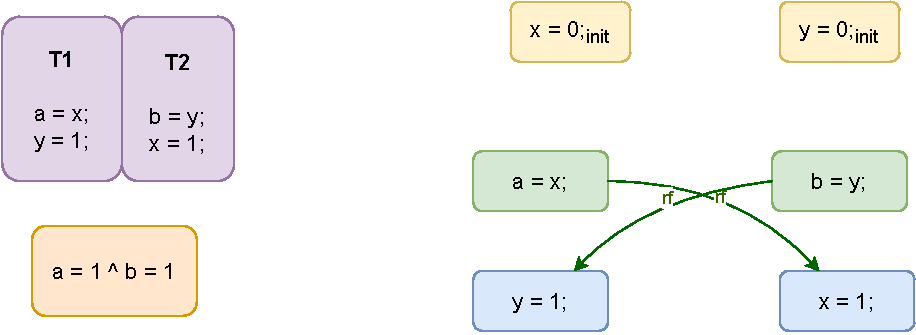
\includegraphics[scale=0.7]{ECMAScriptMemoryModel/ReadsFrom.pdf}
                \caption{An example to show the reads-from relations that are drawn for the example program between read and write events.}
                \label{read-from}
            \end{figure}
            
            %Agent sync with relation
        \subsubsection{Agent-Synchronizes With (\set{ASW})}
        
            A list for each agent that consist of ordered tuples of synchronize events. These tuples specify ordering constraints among agents at different points of execution. So such a list for an agent $k$ would be represented like:  
                \[ASW_k = \{ \langle s_1, s_2 \rangle, \langle s_3, s_4 \rangle ...\}\]
        
            For every pair in the list, the second event belongs to the parent agent and the first belongs to another agent it synchronized with.
                \[  
                    \forall{i,j>0},\ 
                    \langle s_1, s_2 \rangle \in ASW_j 
                    \Rightarrow{} 
                    s_2 \in ael(k)                        
                \]

            The figure below shows an example of this relation among two agents. 
            \begin{figure}[H]
                \centering
                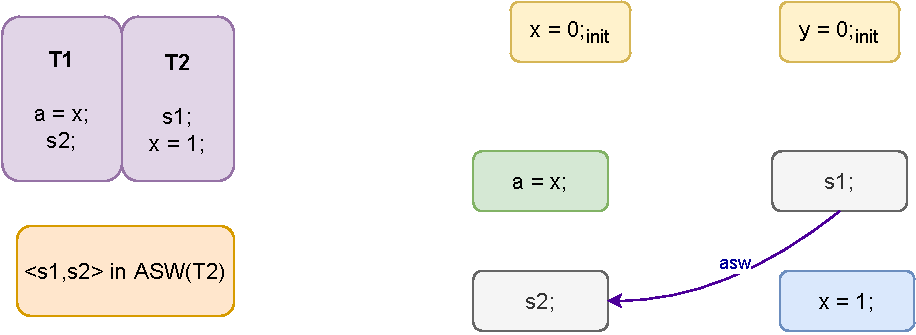
\includegraphics[scale=0.7]{ECMAScriptMemoryModel/AgentSyncWith.pdf}
                \caption{An example to show the reads-from relations that are drawn for the example program between read and write events.}
                \label{agent-sync-with}
            \end{figure}
            \critic{red}{Consider whether figure is needed or not for this sake.}
        
        \critic{blue}{This is analogous to the property that every unlock must be paired with a subsequent lock, which enforces the condition that a lock can be acquired only when it has been released.}